\documentclass[11pt,a4paper]{article}
\usepackage[T1]{fontenc}
\usepackage[utf8]{inputenc}
\usepackage{lmodern}
\usepackage[margin=25mm,headheight=15pt]{geometry}
\usepackage{amsmath,amssymb,amsthm,mathtools}
\usepackage{microtype,booktabs,array,graphicx,xcolor}
\usepackage{enumitem,fancyhdr,hyperref,xurl}
\definecolor{ink}{HTML}{18364A}
\definecolor{accent}{HTML}{096B72}
\hypersetup{colorlinks=true,linkcolor=accent,citecolor=accent,urlcolor=accent,
  pdftitle={Sharp logarithmic remainders for Ford's renewal recurrence},
  pdfauthor={OpenAI, prepared for Vladimir Reshetnikov},
  pdfsubject={Spectral positivity, complete asymptotic expansions, and sharp product bounds}}
\pagestyle{fancy}
\fancyhf{}
\fancyhead[L]{\small\color{ink}Ford's renewal recurrence}
\fancyhead[R]{\small\color{ink}Sharp logarithmic remainders}
\fancyfoot[C]{\thepage}
\renewcommand{\headrulewidth}{0.3pt}
\setlength{\parskip}{4pt}
\setlength{\parindent}{0pt}
\setlength{\emergencystretch}{2em}
\setlist{itemsep=3pt,topsep=4pt}
\numberwithin{equation}{section}
\newtheorem{theorem}{Theorem}[section]
\newtheorem{lemma}[theorem]{Lemma}
\newtheorem{proposition}[theorem]{Proposition}
\newtheorem{corollary}[theorem]{Corollary}
\theoremstyle{definition}
\newtheorem{definition}[theorem]{Definition}
\theoremstyle{remark}
\newtheorem{remark}[theorem]{Remark}
\newcommand{\dd}{\,\mathrm d}
\newcommand{\e}{\mathrm e}
\newcommand{\gE}{\gamma_{\!E}}
\newcommand{\PV}{\operatorname{PV}}
\newcommand{\Li}{\operatorname{Li}}
\newcommand{\Res}{\operatorname{Res}}
\newcommand{\supp}{\operatorname{supp}}
\makeatletter
\let\tableinput\@@input
\makeatother
\title{\color{ink}\bfseries Sharp logarithmic remainders\\
  for Ford's renewal recurrence\\[6pt]
  \large Spectral positivity, complete asymptotic expansions,\\
  and sharp product bounds}
\author{OpenAI\\\small Research manuscript prepared for Vladimir Reshetnikov}
\date{8 October 2026}

\begin{document}
\maketitle
\begin{abstract}
Let $a_j=(j+1)\log(j+1)-j\log j-1$, and let $g_0=1$,
$g_n=\sum_{j=1}^n a_jg_{n-j}$. This recurrence enters the simplex-volume
analysis of values of Euler's totient function. If
$\sum_{j\ge1}a_j\rho^j=1$ and
$\gamma=(\sum_{j\ge1}ja_j\rho^j)^{-1}$, a published estimate bounds
$g_n-\gamma\rho^{-n}$ absolutely by a constant. We prove the sharp
remainder $g_n-\gamma\rho^{-n}\sim-1/(n^2\log^2n)$, and compute its
complete expansion in inverse powers of $\log n$. An exact positive
spectral measure proves strict complete monotonicity of
$E_n=\gamma\rho^{-n}-g_n$ for $n\ge1$, positive definiteness of all
shifted Hankel matrices, and two exact sum rules. We also give a
fully explicit finite-index two-sided bound. A local polylogarithm
identity yields a second expansion in powers of $1/n$ whose coefficients
retain their entire logarithmic dependence; this separates corrections
that every fixed logarithmic truncation would hide. Finally we prove
sharp bounds for the normalized product of the $g_j$, and invert the
renewal-error law to estimate the index needed for a prescribed accuracy.
The proofs are conventional mathematical proofs, supported by independent
high-precision and spectral computations.
\end{abstract}

\smallskip
{\small\textbf{Status.} This is a new research manuscript with internal
independent proof checks, not an externally refereed or Lean-formalized
publication. The exact claims and the limits of the priority search are
recorded in Section~\ref{sec:scope}. No theorem about the full totient
counting function is assumed in these proofs.}

\tableofcontents
\newpage

\section{The problem and the precise improvement}
\label{sec:scope}

The coefficients
\begin{equation}\label{eq:definition-a}
 a_j=(j+1)\log(j+1)-j\log j-1
     =\int_j^{j+1}\log x\,dx\qquad(j\ge1)
\end{equation}
are positive and grow like $\log j$. Set
\begin{equation}\label{eq:definition-g}
 A(z)=\sum_{j\ge1}a_jz^j,\qquad
 g_0=1,\qquad g_n=\sum_{j=1}^n a_jg_{n-j},\qquad
 G(z)=\frac1{1-A(z)}.
\end{equation}
The radius of convergence of $A$ is one. On $[0,1)$ it increases
strictly from zero to infinity. Thus there is a unique $\rho\in(0,1)$
with $A(\rho)=1$. Throughout the paper,
\begin{equation}\label{eq:normalization}
 \gamma=\frac1{\rho A'(\rho)},\qquad
 w_0=\rho^{-1},\qquad
 E_n=\gamma\rho^{-n}-g_n\quad(n\ge1).
\end{equation}
Euler's constant is always $\gE$, to distinguish it from the residue
amplitude $\gamma$. All logarithms are natural. Numerical values, given
only for orientation, are
\[
 \rho=0.542598586098471021959384595779\ldots,
 \qquad \gamma=0.323457534191380676574821548566\ldots.
\]

\subsection{Published baseline and repository connection}

Ford's study of totients uses this recurrence in its simplex-volume
estimates. Lemma~3.7 of the revised paper proves
$|g_n-\gamma\rho^{-n}|\le5$; the following remark records that the
errors for $n\ge1$ are negative, increasing, and summable
\cite[Lemma~3.7 and Remark~1]{Ford}. Ford attributes the simplified
recurrence argument to a solution with Lau \cite{FordLau}.
The present paper starts from those established facts as a comparison;
it proves the new estimates directly.

The same recurrence is defined in the inspected \texttt{openai/math}
totient manuscript, where a continuous counting scale contains
\begin{equation}\label{eq:counting-scale}
 \mathcal G_m(B)=\frac{B^m}{m!\prod_{j=1}^m g_j}.
\end{equation}
We use that definition and its motivation, without using the manuscript's
claims about the arithmetic counting function \cite{OpenAIMath}.
The study also fits the asymptotic-expansion and inversion program in
\texttt{ProveIt} \cite{ProveIt}. Section~\ref{sec:products} gives a
direct, proved consequence for \eqref{eq:counting-scale}.

The priority review inspected Ford's full revised paper and the relevant
repository source. The Ford--Lau item was identified bibliographically,
but its full text was not accessible during preparation. Targeted
searches did not locate the explicit remainder expansion proved here.
This supports a precise claim of a refinement of the inspected published
estimate; it does not establish worldwide first-publication priority.
Spectral measures, Hausdorff moments, renewal generating functions, and
polylogarithm expansions are classical tools.

\subsection{Main conclusions at a glance}

\begin{theorem}[Sharp remainder and all logarithmic orders]
\label{thm:main-log}
For every fixed integer $K\ge0$, as $n\to\infty$,
\begin{equation}\label{eq:main-log}
 E_n=\frac1{n^2}\left\{
    \sum_{k=0}^K\frac{c_k}{(\log n)^{k+2}}
      +O_K\bigl((\log n)^{-K-3}\bigr)\right\},
\end{equation}
where
\begin{equation}\label{eq:main-coeff}
 c_k=(k+1)![u^k]\,
           \frac{(1+u)e^{\gE u}}{\Gamma(1-u)}.
\end{equation}
In particular,
\begin{align}\label{eq:first-coefficients}
 c_0&=1,&c_1&=2,&c_2&=-\frac{\pi^2}{2},\nonumber\\
 c_3&=-2\pi^2-8\zeta(3),&
 c_4&=\frac{\pi^4}{12}-40\zeta(3).
\end{align}
Moreover, $E_n>0$ for every $n\ge1$, and for every $n\ge4096$,
\begin{equation}\label{eq:main-explicit}
 \frac1{200n(n+1)\log^2n}\le E_n
           \le\frac{10}{n(n+1)\log^2n}.
\end{equation}
\end{theorem}

Thus the formerly bounded absolute error actually tends to zero, with
an exact leading constant and an optimal power of $n$ and $\log n$.
After just the first correction,
\[
 g_n=\gamma\rho^{-n}-\frac1{n^2\log^2n}
                   +O\!\left(\frac1{n^2\log^3n}\right).
\]
The new $O$-term is itself sharp: its leading coefficient is $-2$.
The more conservative constants in \eqref{eq:main-explicit} provide
a statement valid from a specified finite index, independently of
any numerical calculation of $\rho$.

\begin{theorem}[Exact moment structure]
\label{thm:main-moment}
There is an explicit positive continuous function $\ell$ on $(0,1)$
such that
\begin{equation}\label{eq:main-moment}
 E_n=\int_0^1 t^{n-1}\ell(t)\,dt\qquad(n\ge1).
\end{equation}
Consequently $(-1)^r\Delta^r E_n>0$ for all $n\ge1$, $r\ge0$,
and every matrix $(E_{a+i+j})_{0\le i,j\le d}$ with $a\ge1$ is
positive definite. The exact sum rules are
\begin{equation}\label{eq:main-sums}
 \sum_{n\ge1}E_n=1-\frac\gamma{1-\rho},\qquad
 \sum_{n\ge1}nE_n=\frac{\gamma\rho}{(1-\rho)^2}.
\end{equation}
\end{theorem}

The restriction $n\ge1$ matters: $g_0-\gamma=1-\gamma>0$ has the
opposite sign. The proof explicitly checks both endpoints of the
spectral measure and excludes an unaccounted singular component.

\subsection{A second, finer expansion}

A fixed truncation of \eqref{eq:main-log} has an error much larger
than $n^{-3}$. To resolve powers of $1/n$ as well, define the ordinary
convergent integrals
\begin{equation}\label{eq:def-Fa}
 F_a(L)=\int_0^\infty
 \frac{y^{a-1}e^{-y}}{(L-\log y-\gE)^2+\pi^2}\,dy
 \qquad(a>0,\ L\in\mathbb R),
\end{equation}
and put
\begin{equation}\label{eq:p2p3}
 p_2=\zeta'(-1)-\frac1{12},\qquad p_3=\zeta'(-2).
\end{equation}
Primes on $F_a$ mean differentiation in $L$.

\begin{theorem}[Expansion retaining all logarithmic dependence]
\label{thm:main-sectors}
Writing $L=\log n$, one has
\begin{align}\label{eq:main-sectors}
 E_n={}&\frac{F_2(L)}{n^2}+\frac{F_3(L)}{2n^3}
   +\frac1{n^4}\left\{\frac{F_4(L)}{12}-p_2F_4'(L)\right\}\nonumber\\
 &-\frac1{n^5}\left(\frac{p_2}{2}+p_3\right)F_5'(L)
   +O\!\left(\frac1{n^6\log^2n}\right).
\end{align}
More generally, an explicit recursion generates the coefficient of
every power $n^{-r-2}$, with remainder
$O_R(n^{-R-3}\log^{-2}n)$ after powers through $n^{-R-2}$.
\end{theorem}

In \eqref{eq:main-sectors}, the $F_a$ are retained as integrals.
Replacing them by a fixed number of inverse-logarithmic terms would
destroy the displayed precision. This distinction is essential when
using the result as an asymptotic expansion in more than one scale.

\subsection{What these theorems do and do not settle}

The main theorem improves a precise analytic component of the totient
method. It also supplies exact inequalities for the entire recurrence,
not merely its tail. The product theorem below determines the first
relative correction to \eqref{eq:counting-scale}; the inverse theorem
quantifies convergence of the associated renewal process.

These conclusions do not, by themselves, improve the error term in an
asymptotic formula for the number of distinct totients. The arithmetic
steps that connect a volume calculation to a count have separate errors.
The present argument neither verifies nor requires the larger claims
in the repository manuscript. This boundary keeps the strengthened
estimate usable as an independently checkable lemma.

% Self-contained mathematical notes for incorporation into the main manuscript.
% No preamble; requires amsmath, amssymb, amsthm.  Prepared independently.

\section{A positive spectral representation of the entire remainder}
\label{sec:spectral-notes}

Put
\[
 a_j=\int_j^{j+1}\log x\,dx\quad(j\ge1),\qquad
 g_0=1,\qquad g_n=\sum_{j=1}^n a_jg_{n-j},
\]
and write $A(z)=\sum_{j\ge1}a_jz^j$ and
$G(z)=\sum_{n\ge0}g_nz^n=1/(1-A(z))$.  Let $\rho\in(0,1)$
be the unique solution of $A(\rho)=1$, put $w_0=\rho^{-1}$, and set
\[
 \gamma=\frac1{\rho A'(\rho)},\qquad
 h(t)=\frac{(1-t)^2}{\log^2t}\quad(0<t<1),\qquad c=2\log2.
\]
The continuous extensions are $h(0)=0$ and $h(1)=1$.  The constant
$\gamma$ is the residue amplitude; Euler's constant is denoted below
by $\gamma_{\!E}$.

\subsection{Elementary integral identities}

The identity
\[
 \frac{1-t}{-\log t}=\int_0^1t^u\,du
\]
gives the useful representation
\begin{equation}
 h(t)=\int_0^1\int_0^1t^{u+v}\,du\,dv.
 \label{eq:spec-h-mixture}
\end{equation}
In particular, Jensen's inequality and $0<t<1$ imply
\begin{equation}
 t\le h(t)\le1.
 \label{eq:spec-h-bounds}
\end{equation}
Direct differentiation of the formula for $a_j$, followed by the
elementary identity $\log(v/u)=\int_0^\infty(e^{-ux}-e^{-vx})\,dx/x$,
gives
\begin{equation}
 a_{j+1}-a_j=\int_0^1t^{j-1}h(t)\,dt\qquad(j\ge1).
 \label{eq:spec-differences}
\end{equation}
For completeness, one may also integrate the right side of
\eqref{eq:spec-h-mixture} first in $t$: it equals
$\int_0^1\int_0^1(j+u+v)^{-1}\,du\,dv$, and the two elementary
integrations yield
$(j+2)\log(j+2)-2(j+1)\log(j+1)+j\log j$.
Consequently
\[
 (1-z)A(z)=a_1z+z^2\int_0^1\frac{h(t)}{1-tz}\,dt,
 \qquad a_1=c-1.
\]
Define, off $[0,1]$,
\begin{equation}
 J(w)=w-c-\int_0^1\frac{h(t)}{w-t}\,dt.
 \label{eq:spec-J}
\end{equation}
Then initially for large $|w|$, and thereafter by analytic continuation,
\begin{equation}
 G(1/w)=\frac{w-1}{J(w)}.
 \label{eq:spec-G-J}
\end{equation}
Finally,
\begin{equation}
 \int_0^1\frac{h(t)}t\,dt
 =\int_0^\infty\frac{(1-e^{-x})^2}{x^2}\,dx=2\log2=c.
 \label{eq:spec-zeroidentity}
\end{equation}
Integration by parts reduces the last integral to
$2\int_0^\infty(e^{-x}-e^{-2x})\,dx/x=2\log2$.

\subsection{A bounded self-adjoint operator}

Work in the Hilbert space
$\mathcal H=\mathbb C\oplus L^2((0,1),h(t)\,dt)$ and define
\begin{equation}
 B(x,f)=\left(cx+\int_0^1f(t)h(t)\,dt,\ x+tf(t)\right).
 \label{eq:spec-operator}
\end{equation}
This is a bounded self-adjoint operator: multiplication by $t$ has
norm at most one and the off-diagonal map is the bounded rank-one
map induced by the constant function.  Moreover,
\begin{equation}
 \langle B(x,f),(x,f)\rangle
 =\int_0^1t h(t)\left|f(t)+\frac{x}{t}\right|^2\,dt\ge0.
 \label{eq:spec-positive}
\end{equation}
The displayed square is integrable because
$\int h(t)/t\,dt=c<\infty$; expanding it gives the preceding
quadratic form exactly.  Thus $B$ is positive.

Let $e_0=(1,0)$.  Solving $(w-B)(x,f)=e_0$ by its second component
gives $f(t)=x/(w-t)$ and hence
\begin{equation}
 \langle(w-B)^{-1}e_0,e_0\rangle=\frac1{J(w)}.
 \label{eq:spec-resolvent}
\end{equation}
By the bounded self-adjoint spectral theorem \cite{Teschl} there is a positive probability measure
$\sigma$, supported in the bounded spectrum of $B$, such that
\begin{equation}
 \frac1{J(w)}=\int\frac{\sigma(dt)}{w-t}.
 \label{eq:spec-measure}
\end{equation}

There is exactly one spectral point above one.  Indeed, on $(1,\infty)$,
\[
 J'(w)=1+\int_0^1\frac{h(t)}{(w-t)^2}\,dt>0,
\]
whereas $J(w)\to-\infty$ as $w\downarrow1$ and $J(w)\to\infty$
as $w\to\infty$.  The unique zero is $w_0=\rho^{-1}$.  The
Schur-complement calculation shows that every real $w\notin[0,1]$
with $J(w)\ne0$ is in the resolvent set.  Positivity excludes negative
spectrum.  Thus
\[
 \operatorname{supp}\sigma\subseteq[0,1]\cup\{w_0\}.
\]
The mass at $w_0$ is
\begin{equation}
 b_0=\sigma(\{w_0\})=\frac1{J'(w_0)},\qquad
 \gamma=\frac{w_0-1}{w_0J'(w_0)}=(1-\rho)b_0.
 \label{eq:spec-atom}
\end{equation}
The final equality can either be read from the residue in
\eqref{eq:spec-G-J} or checked by differentiating that identity.

\subsection{No hidden singular measure}

For $0<t<1$, put
\begin{align}
 R(t)&=t-c-\operatorname{PV}\int_0^1\frac{h(s)}{t-s}\,ds,\\
 J_+(t)&=R(t)+i\pi h(t).
 \label{eq:spec-boundary}
\end{align}
The sign of the imaginary part follows from the upper-half-plane
boundary value of $(w-s)^{-1}$.  Since $h$ is smooth and positive
on compact subintervals of $(0,1)$, the principal value and the
boundary values are continuous there; the convergence from the upper
half-plane is uniform on every smaller compact interval.  Because
$|J_+(t)|\ge\pi h(t)>0$, Stieltjes inversion applied on these
intervals proves absolute continuity, with density
\begin{equation}
 \frac{d\sigma}{dt}=\frac{h(t)}{|J_+(t)|^2}
 \quad(0<t<1).
 \label{eq:spec-density}
\end{equation}
For clarity, this also excludes singular continuous mass in the open
interval: inversion gives the measure of each compact interval as the
integral of the continuous boundary density; such intervals exhaust
$(0,1)$.

Only endpoint atoms remain to be checked.  From
\eqref{eq:spec-zeroidentity}, for $\varepsilon>0$,
\[
 J(-\varepsilon)
 =-\varepsilon\left(1+\int_0^1
            \frac{h(t)}{t(t+\varepsilon)}\,dt\right).
\]
Since $\int_0^1h(t)/t^2\,dt=\infty$,
\begin{equation}
 \sigma(\{0\})
 =\lim_{\varepsilon\downarrow0}\frac{-\varepsilon}{J(-\varepsilon)}=0.
 \label{eq:spec-nozero}
\end{equation}
The divergence follows immediately from
$h(t)\sim1/\log^2t$ at zero.  At the other endpoint,
$J(1+\varepsilon)\to-\infty$, so
\begin{equation}
 \sigma(\{1\})
 =\lim_{\varepsilon\downarrow0}\frac{\varepsilon}{J(1+\varepsilon)}=0.
 \label{eq:spec-noone}
\end{equation}
The isolated atom at $w_0$ contributes zero to this latter limit.
These arguments account for the entire measure:
\begin{equation}
 \sigma=b_0\delta_{w_0}
 +\frac{h(t)}{|J_+(t)|^2}\,\mathbf1_{(0,1)}(t)\,dt.
 \label{eq:spec-fullmeasure}
\end{equation}

\subsection{Exact positive remainder and its consequences}

Since $\sigma$ has total mass one, equations
\eqref{eq:spec-G-J} and \eqref{eq:spec-measure} give
\[
 G(1/w)-1=(w-1)\int\frac{\sigma(dt)}{w-t}-1
         =\int\frac{t-1}{w-t}\,\sigma(dt).
\]
Expanding at infinity is justified by bounded spectral support.
For every integer $n\ge1$,
\begin{equation}
 \boxed{\quad
 E_n:=\gamma\rho^{-n}-g_n
     =\int_0^1t^{n-1}\ell(t)\,dt>0,
 \qquad
 \ell(t)=\frac{(1-t)h(t)}{|J_+(t)|^2}.
 \quad}
 \label{eq:spec-exact-remainder}
\end{equation}
This indexing is essential.  The expression
$\int t^nk(t)\,dt$ with $k=\ell/t$ is equivalent for $n\ge1$,
but it must not be extended to $n=0$: the corresponding density is
not integrable at zero.  Indeed $J(-\varepsilon)\to0^-$ by dominated
convergence in \eqref{eq:spec-J} and \eqref{eq:spec-zeroidentity}, so
$G(-1/\varepsilon)-1\to+\infty$ in
\eqref{eq:spec-G-J}.  Its Cauchy representation is a bounded isolated
pole term plus $\int_0^1\ell(t)/(t+\varepsilon)\,dt$; monotone
convergence proves $\int_0^1\ell(t)/t\,dt=\infty$.
The exact generating-function identity is
\begin{equation}
 G(z)=1+\frac{\gamma\rho^{-1}z}{1-z/\rho}
             -z\int_0^1\frac{\ell(t)}{1-tz}\,dt.
 \label{eq:spec-regularized-generating}
\end{equation}

The representation proves strict complete monotonicity:
\begin{equation}
 (-1)^k\Delta^k E_n
 =\int_0^1t^{n-1}(1-t)^k\ell(t)\,dt>0
 \qquad(n\ge1,\ k\ge0),
 \label{eq:spec-complete-monotone}
\end{equation}
where $\Delta E_n=E_{n+1}-E_n$.  Every finite Hankel matrix
$(E_{r+i+j})_{0\le i,j\le m}$ is positive definite when $r\ge1$:
for any nonzero real polynomial $P(t)=\sum_{i=0}^mc_it^i$,
\[
 \sum_{i,j=0}^mc_ic_jE_{r+i+j}
 =\int_0^1t^{r-1}P(t)^2\ell(t)\,dt>0.
\]
In particular $E_{n+1}^2<E_nE_{n+2}$.  These are exact finite-$n$
statements, independent of any asymptotic expansion.

Several exact sum rules are also available.  Comparing the coefficient
of $1/w$ gives
\begin{equation}
 \int_0^1\ell(t)\,dt=\gamma\rho^{-1}-a_1<1.
 \label{eq:spec-massell}
\end{equation}
Monotone convergence and the total mass of $\sigma$ give
\begin{equation}
 \sum_{n=1}^\infty E_n
 =\int_0^1\frac{\ell(t)}{1-t}\,dt
 =1-b_0=1-\frac\gamma{1-\rho}.
 \label{eq:spec-sum0}
\end{equation}
Letting $w\downarrow1$ in \eqref{eq:spec-measure} shows that
$\int_0^1(1-t)^{-1}\,\sigma(dt)=b_0/(w_0-1)$: the continuous
part increases monotonically and the left side $1/J(w)$ tends to zero,
while the isolated-pole term tends to $-b_0/(w_0-1)$.  Consequently
\begin{equation}
 \sum_{n=1}^\infty nE_n
 =\int_0^1\frac{\ell(t)}{(1-t)^2}\,dt
 =\frac{b_0}{w_0-1}
 =\frac{\gamma\rho}{(1-\rho)^2}.
 \label{eq:spec-sum1}
\end{equation}

\section{Explicit finite-index bounds and the sharp leading scale}
\label{sec:spectral-bounds-notes}

We next prove actual numerical constants without needing certified
quadrature for the spectral density.  They are deliberately conservative;
the exact integral \eqref{eq:spec-exact-remainder} supports much tighter
numerical enclosures.

\subsection{The logarithmic endpoint constant}

Define
\[
 C=\int_0^1\frac{h(s)-1}{1-s}\,ds.
\]
With $s=e^{-x}$ this becomes
\[
 C=\int_0^\infty\left(
       \frac{e^{-x}-e^{-2x}}{x^2}-\frac1{e^x-1}\right)dx.
\]
Writing $\operatorname{E}_1(a)=\int_a^\infty e^{-x}\,dx/x$,
integration by parts after a cutoff $\varepsilon$ gives
\[
 C=\lim_{\varepsilon\downarrow0}
 \left\{
 \frac{e^{-\varepsilon}-e^{-2\varepsilon}}\varepsilon
 -\operatorname{E}_1(\varepsilon)
 +2\operatorname{E}_1(2\varepsilon)
 +\log(1-e^{-\varepsilon})\right\}.
\]
The standard integral definition
$\gamma_{\!E}=-\lim_{\varepsilon\downarrow0}
 (\operatorname{E}_1(\varepsilon)+\log\varepsilon)$ therefore yields
\begin{equation}
 C=1-2\log2-\gamma_{\!E}.
 \label{eq:spec-Cconstant}
\end{equation}
Only $0<\gamma_{\!E}<1$ is needed for the explicit bounds below.
These inequalities follow, for example, from
\[
 \gamma_{\!E}=\int_0^1\frac{1-e^{-x}}x\,dx
                  -\int_1^\infty\frac{e^{-x}}x\,dx.
\]

Put $r(s)=(h(s)-1)/(1-s)$ and extend it at one by $r(1)=-1$.
By \eqref{eq:spec-h-bounds}, $-1\le r(s)\le0$.  If $t=1-u$,
then a direct decomposition $h(s)=1+(1-s)r(s)$ gives
\begin{equation}
 R(1-u)=\log u+\gamma_{\!E}+\eta(u),\qquad
 \eta(u)=-u-\log(1-u)
       -u\operatorname{PV}\int_0^1\frac{r(s)}{1-u-s}\,ds.
 \label{eq:spec-etaidentity}
\end{equation}
Here $R$ is the real part in \eqref{eq:spec-boundary}.

We record explicit estimates for the last principal value.  From
\eqref{eq:spec-h-mixture}, for $s\in[1/4,1]$,
$|h''(s)|\le32$: indeed $|q(q-1)|\le2$ for $0\le q\le2$ and
$s^{q-2}\le16$.  Since $r$ is the negative average of $h'$ over
$[s,1]$, this implies $|r'(s)|\le16$ on that interval.  For
$t\in[1/2,1)$,
\[
 \operatorname{PV}\int_0^1\frac{r(s)}{t-s}\,ds
 =r(t)\log\frac{t}{1-t}
       +\int_0^1\frac{r(s)-r(t)}{t-s}\,ds.
\]
The integral over $[0,1/4]$ has absolute value at most one; the
remaining part has absolute value at most $16(3/4)=12$.  Therefore,
with $L=\log(1/u)$ and $0<u\le1/2$,
\begin{equation}
 |\eta(u)|\le u(L+14).
 \label{eq:spec-eta-bound}
\end{equation}
We used $0\le-u-\log(1-u)\le u^2$ for $u\le1/2$.
In particular,
\begin{equation}
 J_+(1-u)=\log u+\gamma_{\!E}+i\pi
                  +O(u\log(1/u)),
 \qquad
 \ell(1-u)\sim\frac{u}{\log^2(1/u)}.
 \label{eq:spec-local-equivalence}
\end{equation}

\subsection{Two-sided density bounds with actual constants}

For $0<u\le e^{-4}$, $L\ge4$ and
$u(L+14)\le18e^{-4}<1/3$.  Using $0<\gamma_{\!E}<1$,
\eqref{eq:spec-eta-bound} implies
\[
 \frac23L\le |R(1-u)|\le\frac43L.
\]
Also $h(1-u)\ge1-u>1/2$, $h(1-u)\le1$, and
$\pi h(1-u)\le\pi<L$.  Hence
\begin{equation}
 \boxed{\qquad
 \frac9{50}\frac{u}{\log^2(1/u)}
 \le\ell(1-u)\le
 \frac94\frac{u}{\log^2(1/u)}
 \quad(0<u\le e^{-4}).
 \qquad}
 \label{eq:spec-explicit-density}
\end{equation}

\subsection{A fully explicit finite-index theorem}

For every integer $n\ge4096$,
\begin{equation}
 \boxed{\qquad
 \frac{1}{200\,n(n+1)\log^2n}
 \le \gamma\rho^{-n}-g_n
 \le\frac{10}{n(n+1)\log^2n}.
 \qquad}
 \label{eq:spec-explicit-n}
\end{equation}
To prove the upper bound, split the integral in
\eqref{eq:spec-exact-remainder} at $u=n^{-1/2}\le e^{-4}$.
On the part $u\le n^{-1/2}$, $\log(1/u)\ge\tfrac12\log n$, so
\[
 \int_0^{n^{-1/2}}(1-u)^{n-1}\ell(1-u)\,du
 \le\frac9{\log^2n}\int_0^1(1-u)^{n-1}u\,du
 =\frac9{n(n+1)\log^2n}.
\]
On the complement use $\int\ell\le1$, a consequence of the
probability measure $\sigma$:
\[
 \int_{n^{-1/2}}^1(1-u)^{n-1}\ell(1-u)\,du
 \le e^{-\sqrt n+1/\sqrt n}
 \le\frac1{n(n+1)\log^2n}.
\]
For the last elementary inequality set $r=\sqrt n\ge64$.  The
difference between the logarithms of the two sides, with signs reversed,
is
\[
 r-r^{-1}-4\log r-\log(1+r^{-2})-2\log(2\log r).
\]
It is positive at $r=64$ (use $\log64<5$ and $\log10<3$), and its
derivative is positive for $r\ge64$.

For the lower bound restrict to $1/(2n)\le u\le1/n$.  On that
interval, $(1-u)^{n-1}\ge e^{-1}>1/3$ and
$\log(1/u)\le\log(2n)\le2\log n$.  Equation
\eqref{eq:spec-explicit-density} gives
\[
 E_n\ge\frac{9}{600\log^2n}
               \int_{1/(2n)}^{1/n}u\,du
      =\frac9{1600\,n^2\log^2n}
      \ge\frac1{200\,n(n+1)\log^2n}.
\]
No numerical root approximation, numerical principal value, or numerical
integration is used in \eqref{eq:spec-explicit-n}.

A weaker bound valid at every $n\ge2$ follows from
$|J_+(t)|^2\ge\pi^2h(t)^2$ and $h(t)\ge t$:
\begin{equation}
 0<E_n\le\frac1{\pi^2 n(n-1)}\qquad(n\ge2).
 \label{eq:spec-global-simple}
\end{equation}

\subsection{Sharp asymptotic constant}

The same estimates give
\begin{equation}
 \boxed{\qquad
 E_n\sim\frac1{n^2\log^2n}.
 \qquad}
 \label{eq:spec-leading}
\end{equation}
Here are details avoiding an implicit Tauberian hypothesis.  The part
$u\ge n^{-1/2}$ is negligible after multiplication by $n^2\log^2n$,
as just shown.  In the remaining integral put $v=nu$.  For each fixed
$v>0$, \eqref{eq:spec-local-equivalence} gives
\[
 n^2\log^2n\,(1-v/n)^{n-1}\ell(1-v/n)\,\frac{dv}{n}
 \longrightarrow ve^{-v}\,dv.
\]
For $v\le\sqrt n$, \eqref{eq:spec-explicit-density} bounds the
integrand by $9ve^{-v/2}$ for all sufficiently large $n$.  Dominated
convergence applies, and $\int_0^\infty ve^{-v}\,dv=1$.

Thus the error has a fixed negative sign in $g_n-\gamma\rho^{-n}$,
its absolute order $n^{-2}(\log n)^{-2}$ cannot be improved, and its
entire finite-index shape is constrained by a positive Hausdorff moment
representation.

\section{Complete expansions in two asymptotic scales}
\label{sec:expansions}

The positive measure resolves global singularities and signs. We now analyze
its endpoint with enough precision to recover every inverse-logarithmic
coefficient and every fixed algebraic order. The first expansion keeps only
powers of $1/\log n$; the second retains these logarithmic effects inside
convergent integral functions before expanding in $1/n$.

We use $J$, $h$, and $\ell$ from
Section~\ref{sec:spectral-notes}. The boundary value is
$J_+(t)=R(t)+i\pi h(t)$. All truncation indices and all parameters
$a>0$ below are fixed while $n$ or $L$ tends to infinity.

\subsection{The exact analytic endpoint correction}

The stronger identity is
\begin{equation}\label{exp:exactP}
 \frac{J(e^{-s}+i0)}{h(e^{-s})}
 =\log s+\gE+P(s)+i\pi,\qquad 0<s<2\pi,
\end{equation}
where the real-analytic function $P$ has the convergent expansion
\begin{equation}\label{exp:P}
 P(s)=\frac{s^2}{4\sinh^2(s/2)}-1
       +\sum_{k=0}^{\infty}\zeta'(-1-k)\frac{s^{k+2}}{k!}.
\end{equation}
The assertion for the whole interval $(0,2\pi)$ means continuation of the
convergent Taylor expression there. Its local use near zero is all that is
needed below. In particular,
\[
 P(s)=p_2s^2+p_3s^3+p_4s^4+O(s^5),
 \quad
 p_2=\zeta'(-1)-\frac1{12},\quad
 p_3=\zeta'(-2),\quad
 p_4=\frac12\zeta'(-3)+\frac1{240}.
\]

Here is a derivation fixing the signs. Define
\[
 \mathcal B(z)=\sum_{m\geq1}m\log m\,z^m
             =-\left.\partial_\nu\operatorname{Li}_\nu(z)\right|_{\nu=-1}.
\]
The coefficients of $A(z)=\sum_{j\geq1}a_jz^j$ give
\[
 A(z)=(z^{-1}-1)\mathcal B(z)-\frac z{1-z},
 \qquad
 (1-z)(1-A(z))=1-\frac{(1-z)^2}{z}\mathcal B(z).
\]
Differentiate the classical convergent polylogarithm expansion \cite[25.12.12]{DLMF}
\[
 \operatorname{Li}_\nu(e^{-u})
 =\Gamma(1-\nu)u^{\nu-1}
  +\sum_{k\geq0}\zeta(\nu-k)\frac{(-u)^k}{k!},\qquad |u|<2\pi,
\]
at $\nu=-1$, using the principal logarithm away from the negative real axis.
It gives
\[
 \mathcal B(e^{-u})
 =\frac{1-\gE-\log u}{u^2}
  -\sum_{k\geq0}\zeta'(-1-k)\frac{(-u)^k}{k!}.
\]
For $w=e^u$ one has
$J(w)=w(1-w^{-1})(1-A(w^{-1}))$.
Substitute the last display and then let $u\to-s+i0$.
Since $\log(-s+i0)=\log s+i\pi$ and
\[
 h(e^{-s})=e^{-s}\frac{4\sinh^2(s/2)}{s^2},
\]
the result is \eqref{exp:exactP}--\eqref{exp:P}.
The lower boundary has $-i\pi$. The positive sign on the upper boundary also
agrees with the direct Sokhotski--Plemelj formula for $J$.

\subsection{A Laplace form and the correct scale of the first correction}

Let $L=\log n$ and, for $a>0$, define
\begin{equation}\label{exp:Fa}
 F_a(L)=\int_0^\infty
     \frac{y^{a-1}e^{-y}}
      {(L-\log y-\gE)^2+\pi^2}\,dy.
\end{equation}
These functions are positive, finite, and differentiable to every order on
the real axis. The denominator is bounded below by $\pi^2$.
In \eqref{eq:spec-exact-remainder} the change of variables $t=e^{-s}$ is especially useful:
\[
 E_n=\int_0^\infty e^{-ns}\ell(e^{-s})\,ds.
\]
For sufficiently small positive $s$, \eqref{exp:exactP} yields the exact
local density expression
\begin{equation}\label{exp:laplacedensity}
 \ell(e^{-s})
 =\frac{s^2}{1-e^{-s}}
     \frac1{(\log s+\gE+P(s))^2+\pi^2}.
\end{equation}
The part of the original moment integral with $t\leq e^{-\delta}$ is
$O(e^{-(n-1)\delta})$, since $\ell$ is integrable. Thus only a fixed
neighbourhood of $s=0$ enters any of the algebraic orders below.

The expansion $P(s)=O(s^2)$ in \eqref{exp:exactP} gives
\[
 \ell(e^{-s})
 =\frac{s+s^2/2}{(\log s+\gE)^2+\pi^2}
  +O\left(\frac{s^3}{(\log s+\gE)^2+\pi^2}\right).
\]
Consequently
\begin{equation}\label{exp:twosectors}
 E_n=\frac{F_2(L)}{n^2}+\frac{F_3(L)}{2n^3}
           +O\left(\frac1{n^4L^2}\right).
\end{equation}
In particular the first relative correction in powers of $1/n$ is positive.

For comparison, the direct $t$-variable model satisfies the weaker but useful
bound
\[
 E_n=\int_0^1\frac{t^{n-1}(1-t)}
       {(\log(1-t)+\gE)^2+\pi^2}\,dt
         +O\left(\frac1{n^3\log^2n}\right).
\]
Its error has a genuine $n^{-3}\log^{-2}n$ contribution; changing to the
Laplace variable incorporates the corresponding first correction cleanly.

\subsection{Every fixed algebraic order, retaining the logarithmic dependence}

Put
\[
 f(V)=\frac1{V^2+\pi^2},\qquad b(s)=\frac{s}{1-e^{-s}},
 \qquad
 b(s)f(V+P(s))=\sum_{r\geq0}Q_r(V)s^r.
\]
The last identity defines $Q_r$ by Taylor expansion in $s$ while $V$ is held
fixed. Each $Q_r$ is a finite linear combination of derivatives of $f$, with
constants obtained from the Bernoulli coefficients of $b$ and the Taylor
coefficients of $P$. Explicitly,
\begin{align*}
 Q_0&=f,&Q_1&=\tfrac12f,\\
 Q_2&=\tfrac1{12}f+p_2f',&
 Q_3&=(p_2/2+p_3)f',\\
 Q_4&=-\tfrac1{720}f+(p_2/12+p_3/2+p_4)f'
                    +\tfrac12p_2^2 f''.
\end{align*}
Define the coefficient functions
\[
 \Psi_r(L)=\int_0^\infty
   y^{r+1}e^{-y}Q_r(\log y-L+\gE)\,dy.
\]
Then, for every fixed integer $R\geq0$,
\begin{equation}\label{exp:powerexpansion}
 E_n=\sum_{r=0}^{R}\frac{\Psi_r(\log n)}{n^{r+2}}
       +O_R\left(\frac1{n^{R+3}\log^2n}\right).
\end{equation}

Here is a uniform remainder proof. Choose a small fixed circle
$|\xi|=r_0<2\pi$ on which $b$ and $P$ are analytic, and let
$M=\sup_{|\xi|\leq r_0}|P(\xi)|$.
For real $|V|>2(M+\pi+1)$, the function
$b(\xi)f(V+P(\xi))$ is analytic in that disk and is bounded by $C/V^2$.
Cauchy's estimate for its Taylor remainder, for $0<s<r_0/2$, gives
\[
 b(s)f(V+P(s))-\sum_{r=0}^{R}Q_r(V)s^r
       =O_R(s^{R+1}/V^2).
\]
Choose $\delta$ small enough that this applies to
$V=\log s+\gE$ for $0<s<\delta$.
Multiplication by $s$ in \eqref{exp:laplacedensity} makes the local density
error $O_R(s^{R+2}/\log^2s)$.
For each fixed $m\geq0$,
\[
 \int_0^\delta e^{-ns}\frac{s^m}{1+\log^2s}\,ds
       =O_m(n^{-m-1}\log^{-2}n).
\]
Indeed, on $s\leq n^{-1/2}$ the denominator is at least a constant times
$\log^2n$, and the remaining part is exponentially small in $\sqrt n$.
This proves the remainder in \eqref{exp:powerexpansion}.
Finally, every $Q_r$ is bounded on the real axis and decays as $O_r(V^{-2})$,
so extending the coefficient integrals from $y<n\delta$ to $y<\infty$
adds only exponentially small errors.

With the convention that a prime on $F_a$ means differentiation in $L$,
the first four power sectors are therefore
\begin{align}\label{exp:fourpowers}
 E_n={}&\frac{F_2(L)}{n^2}+\frac{F_3(L)}{2n^3}
 +\frac1{n^4}\left\{\frac{F_4(L)}{12}-p_2F_4'(L)\right\}\notag\\
 &\quad-\frac{p_2/2+p_3}{n^5}F_5'(L)
       +O\left(\frac1{n^6L^2}\right).
\end{align}
The minus signs in the derivative terms are forced by
$V=\log y-L+\gE$; $f$ is even but $f'$ is odd.
The $n^{-6}$ coefficient, if wanted, is
\[
 -\frac{F_6}{720}-(p_2/12+p_3/2+p_4)F_6'
                       +\frac{p_2^2}{2}F_6''.
\]
It can be included with an $O(n^{-7}L^{-2})$ remainder by taking $R=4$.

\paragraph{Essential scope distinction.}
In \eqref{exp:powerexpansion}, the functions $\Psi_r$ (or the $F_a$ in
\eqref{exp:fourpowers}) remain intact. Truncating the inverse-logarithmic
expansion of the leading sector at any fixed order produces an error larger
than every later fixed power of $1/n$. A finite rectangular double sum does
not inherit the remainder in \eqref{exp:powerexpansion}.

\subsection{Every fixed inverse-logarithmic order}

For $k\geq0$ put
\[
 q_k(U)=\frac{(U+i\pi)^{k+1}-(U-i\pi)^{k+1}}{2i\pi}
       =\sum_{j=0}^{\lfloor k/2\rfloor}
          (-1)^j\binom{k+1}{2j+1}\pi^{2j}U^{k-2j}.
\]
For every fixed $a>0$ and $K\geq0$,
\begin{equation}\label{exp:logexpansion}
 F_a(L)=\Gamma(a)\sum_{k=0}^{K}\frac{c_{a,k}}{L^{k+2}}
                +O_{a,K}(L^{-K-3}),\qquad L\to\infty,
\end{equation}
where
\[
 c_{a,k}=\frac1{\Gamma(a)}\int_0^\infty
       y^{a-1}e^{-y}q_k(\log y+\gE)\,dy.
\]
To prove the remainder, split the integral into
$y<e^{-L/2}$, $e^{-L/2}\leq y\leq e^{L/2}$, and $y>e^{L/2}$.
The outer parts, including the tails of the proposed coefficients, are
smaller than every fixed inverse power of $L$.
On the middle part expand
\[
 \frac1{(L-U)^2+\pi^2}
 =\frac1{2i\pi}\left\{\frac1{L-U-i\pi}-\frac1{L-U+i\pi}\right\}.
\]
For sufficiently large $L$, $|U\pm i\pi|\leq3L/4$ there.
The finite geometric expansion through the required order has a remainder
bounded by $C_K L^{-K-3}(1+|U|^{K+2})$.
All logarithmic moments against $y^{a-1}e^{-y}$ are finite, proving
\eqref{exp:logexpansion}.

The coefficient generating function has a particularly simple form:
\begin{equation}\label{exp:coeffgen}
 \sum_{k\geq0}\frac{c_{a,k}}{(k+1)!}z^k
 =\frac{\Gamma(a+z)}{\Gamma(a)}e^{\gE z}
          \frac{\sin\pi z}{\pi z}.
\end{equation}
This follows first for small $z$ by integrating
$\sum q_k(U)z^k/(k+1)!=e^{Uz}\sin(\pi z)/(\pi z)$.
For a positive integer $a$ the reflection formula rewrites it as
\[
 \sum_{k\geq0}\frac{c_{a,k}}{(k+1)!}z^k
 =\left\{\prod_{j=1}^{a-1}(1+z/j)\right\}
                       \frac{e^{\gE z}}{\Gamma(1-z)}.
\]
The right-hand side is entire. This is a coefficient-generation statement;
it does not assert convergence of the asymptotic inverse-log series.

For the leading sector, $a=2$, let $c_k=c_{2,k}$. Then
\begin{equation}\label{exp:maincoeffgen}
 \sum_{k\geq0}\frac{c_k}{(k+1)!}z^k
 =(1+z)\frac{e^{\gE z}}{\Gamma(1-z)}
 =(1+z)\exp\left\{-\sum_{m\geq2}\frac{\zeta(m)}m z^m\right\}.
\end{equation}
The displayed exponential identity holds in $|z|<1$; the preceding gamma
quotient gives its entire continuation. The first five coefficients are
\[
 c_0=1,\quad c_1=2,\quad c_2=-\frac{\pi^2}{2},\quad
 c_3=-2\pi^2-8\zeta(3),\quad
 c_4=\frac{\pi^4}{12}-40\zeta(3).
\]
For a recursive implementation set $b_0=1$, $b_1=0$ and
\[
 b_k=-\frac1k\sum_{m=2}^{k}\zeta(m)b_{k-m}\quad(k\geq2),
 \qquad c_k=(k+1)!(b_k+b_{k-1}),
\]
where $b_{-1}=0$. Thus, for every fixed $K$,
\begin{equation}\label{exp:mainresult}
 g_n=\gamma\rho^{-n}
 -\frac1{n^2}\sum_{k=0}^{K}\frac{c_k}{\log^{k+2}n}
 +O_K\left(\frac1{n^2\log^{K+3}n}\right).
\end{equation}
In particular,
\[
 g_n-\gamma\rho^{-n}
 =-\frac1{n^2\log^2n}
 \left\{1+\frac2{\log n}-\frac{\pi^2}{2\log^2n}
       -\frac{2\pi^2+8\zeta(3)}{\log^3n}
       +O(\log^{-4}n)\right\}.
\]
For the $n^{-3}$ sector in \eqref{exp:twosectors}, the normalized first
coefficients are
\[
 \frac12F_3(L)=\frac1{L^2}
 \left\{1+\frac3L+\frac{3-\pi^2/2}{L^2}
              -\frac{3\pi^2+8\zeta(3)}{L^3}+O(L^{-4})\right\}.
\]
Their generating function is
$(1+z)(1+z/2)e^{\gE z}/\Gamma(1-z)$.


\section{Products and the continuous totient counting scale}
\label{sec:products}

The recurrence enters \eqref{eq:counting-scale} multiplicatively, so
an additive estimate should be transported through the product with
its sign and its first correction intact. Define
\begin{equation}\label{eq:product-definitions}
 \delta_n=\frac{\rho^n E_n}{\gamma},\qquad
 P_m=\prod_{j=1}^m\frac{g_j}{\gamma\rho^{-j}}
     =\prod_{j=1}^m(1-\delta_j).
\end{equation}
Positivity of $g_j$ and the exact moment representation give
$0<\delta_j<1$. Moreover,
\begin{equation}\label{eq:delta-geometric}
 0<\delta_{j+1}<\rho\delta_j,
\end{equation}
because $E_{j+1}<E_j$. Hence $P_m$ decreases to a strictly positive
constant
\begin{equation}\label{eq:product-constant}
 C_*:=\prod_{j=1}^\infty(1-\delta_j)\in(0,1).
\end{equation}
Strict positivity follows from convergence of $\sum\delta_j$ and the
fact that none of the individual factors vanishes.

\begin{theorem}[Sharp product tail]
\label{thm:product}
For every fixed $K\ge0$, set $n=m+1$ and $L=\log n$. Then
\begin{equation}\label{eq:product-asymptotic}
 \log\frac{P_m}{C_*}
 =\frac{\rho^n}{\gamma(1-\rho)n^2}
    \left\{\sum_{k=0}^K\frac{c_k}{L^{k+2}}
                     +O_K(L^{-K-3})\right\}.
\end{equation}
In particular,
\begin{equation}\label{eq:product-leading}
 P_m=C_*\left[1+
   \frac{\rho^{m+1}}{\gamma(1-\rho)(m+1)^2\log^2(m+1)}
       \left(1+\frac2{\log(m+1)}+O(\log^{-2}(m+1))\right)
        \right].
\end{equation}
\end{theorem}

\begin{proof}
Write
\[
 T_m=\sum_{j=m+1}^\infty\delta_j,\qquad
 R_m=\sum_{j=m+1}^\infty[-\log(1-\delta_j)-\delta_j].
\]
Then $\log(P_m/C_*)=T_m+R_m$. The elementary power series for
$-\log(1-x)$ and \eqref{eq:delta-geometric} give
\begin{equation}\label{eq:log-remainder-bound}
 0\le R_m\le
 \frac{\delta_n^2}{2(1-\delta_n)(1-\rho^2)},\qquad n=m+1.
\end{equation}
Tonelli's theorem applied to the positive moment representation gives
the exact identity
\begin{equation}\label{eq:product-tail-integral}
 T_m=\frac{\rho^n}{\gamma}
       \int_0^1\frac{t^{n-1}\ell(t)}{1-\rho t}\,dt.
\end{equation}
Put $\beta=\rho/(1-\rho)$ and
\begin{equation}\label{eq:D-def}
 D_{n,r}=(-1)^r\Delta^r E_n
        =\int_0^1t^{n-1}(1-t)^r\ell(t)\,dt.
\end{equation}
Since $(1-\rho t)^{-1}=(1-\rho)^{-1}
[1-\beta(1-t)/(1+\beta(1-t))]$,
\begin{equation}\label{eq:tail-first-sandwich}
 \frac{\rho^n}{\gamma(1-\rho)}(E_n-\beta D_{n,1})
 \le T_m\le\frac{\rho^n E_n}{\gamma(1-\rho)}.
\end{equation}
The same endpoint argument that gives the main theorem yields
$D_{n,1}=O(n^{-3}\log^{-2}n)$; a proof with all coefficients is
given in Section~\ref{sec:additional-consequences}. Thus replacing
$(1-\rho t)^{-1}$ by $(1-\rho)^{-1}$ costs an extra factor $1/n$.
For every fixed $K$, this error and \eqref{eq:log-remainder-bound}
are absorbed by the last term of \eqref{eq:product-asymptotic}.
Exponentiating proves \eqref{eq:product-leading}.
\end{proof}

\subsection{Finite, computable two-sided bounds for the product constant}

The integral proof gives more than an asymptotic notation. For $n=m+1$,
let
\begin{align}\label{eq:product-finite-bounds}
 U_m&=\frac{\delta_n}{1-\rho}
       +\frac{\delta_n^2}{2(1-\delta_n)(1-\rho^2)},\nonumber\\
 L_m&=\max\left\{\delta_n,
   \frac{\rho^n}{\gamma(1-\rho)}(E_n-\beta D_{n,1})\right\}.
\end{align}
Every $m\ge0$ satisfies
\begin{equation}\label{eq:C-enclosure}
 \boxed{\qquad P_m e^{-U_m}\le C_*\le P_m e^{-L_m}.\qquad}
\end{equation}
The additional lower bound $T_m\ge\delta_n$ used here follows directly
from its defining positive sum. These formulas involve just finitely
many recurrence terms and the two scalar constants $\rho,\gamma$.
They become certified numerical enclosures when those inputs are
enclosed by outward-rounded interval arithmetic. The supplied
high-precision computations are diagnostics, and are not described
as interval certificates.

There is a systematic refinement. The exact finite geometric identity
gives, for every $r\ge1$,
\begin{align}\label{eq:alternating-tail}
 T_m={}&\frac{\rho^n}{\gamma(1-\rho)}
       \sum_{j=0}^{r-1}(-\beta)^jD_{n,j}
       +\mathcal R_{m,r},\nonumber\\
 0<&(-1)^r\mathcal R_{m,r}
       \le\frac{\rho^n\beta^r}{\gamma(1-\rho)}D_{n,r}.
\end{align}
No convergence of an infinite geometric series with ratio $\beta$ is
being used: $\beta>1$ is allowed. The signed remainder is the exact
integral with factor $(1+\beta(1-t))^{-1}$. For each fixed $r$,
$D_{n,r}=O_r(n^{-r-2}\log^{-2}n)$, so successive bounds resolve
successive powers of $1/n$.

\subsection{Effect on the counting scale}

From the definition of $P_m$ one obtains the exact algebraic identity
\begin{equation}\label{eq:counting-scale-product}
 \mathcal G_m(B)
 =\frac{B^m\rho^{m(m+1)/2}}{m!\gamma^m C_*}
       \exp\left(-\log\frac{P_m}{C_*}\right).
\end{equation}
It follows that the approximation obtained by replacing $P_m$ with
$C_*$ is an upper approximation. Its relative correction has the
sharp size
\begin{equation}\label{eq:counting-correction}
 \frac{\rho^{m+1}}{
   \gamma(1-\rho)(m+1)^2\log^2(m+1)}.
\end{equation}
This improves the product-tail estimate $O(\rho^m)$ obtainable from
a bounded absolute recurrence error by the factor
$m^{-2}\log^{-2}m$, and determines its leading constant and sign.
It is a statement about the scale \eqref{eq:counting-scale}. It does
not identify or eliminate independent arithmetic errors in a totient
counting argument.

\section{A renewal process and inversion of its convergence rate}
\label{sec:renewal-inversion}

Define a probability distribution on the positive integers by
\begin{equation}\label{eq:renewal-law}
 p_j=a_j\rho^j\quad(j\ge1).
\end{equation}
Its total mass is $A(\rho)=1$ and its mean is
$\sum jp_j=1/\gamma$. For independent positive integer-valued
increments with this law, let $u_n$ be the probability that a renewal
occurs at time $n$, with $u_0=1$. Splitting according to the first
increment gives
$u_n=\sum_{j=1}^n p_ju_{n-j}$, so
\begin{equation}\label{eq:renewal-u}
 u_n=\rho^n g_n,\qquad
 \gamma-u_n=\rho^n E_n\quad(n\ge1).
\end{equation}
Thus the renewal probabilities increase strictly to $\gamma$ from
time one onward, and
\begin{equation}\label{eq:renewal-sharp}
 \gamma-u_n=
 \frac{\rho^n}{n^2\log^2n}
 \left(1+\frac2{\log n}-\frac{\pi^2}{2\log^2n}
                         +O(\log^{-3}n)\right).
\end{equation}
The exponential rate is exactly $\rho$:
$\lim(\gamma-u_n)^{1/n}=\rho$. No bound $O(r^n)$ with $r<\rho$
can hold. The extra polynomial and logarithmic factors describe the
behavior at this exact exponential rate.

The moment formula also extends the error to real indices:
\begin{equation}\label{eq:continuous-error}
 E(x)=\int_0^1t^{x-1}\ell(t)\,dt,
 \qquad \delta(x)=\frac{\rho^xE(x)}\gamma\qquad(x\ge1).
\end{equation}
It is continuous for $x\ge1$, smooth for $x>1$, and strictly decreasing
to zero. All the asymptotic proofs above remain valid for real
$x\to\infty$.

\begin{theorem}[Inverse error law]
\label{thm:inverse}
Let $0<\varepsilon<\delta(1)$, and let $x_\varepsilon$ be the
unique real solution of $\delta(x_\varepsilon)=\varepsilon$.
Write
\[
 a=\log(1/\rho),\qquad
 B=\log(1/\varepsilon),\qquad T=\log B,\qquad c=\log a.
\]
Then as $\varepsilon\downarrow0$,
\begin{align}\label{eq:inverse-expansion}
 ax_\varepsilon={}&B-2T-2\log T+2c-\log\gamma
             +\frac{2c+2}{T}\nonumber\\
 &+\frac{c^2+2c-\pi^2/2-2}{T^2}+O(T^{-3}).
\end{align}
The least positive integer index with relative renewal error at most
$\varepsilon$ is exactly $\lceil x_\varepsilon\rceil$.
\end{theorem}

\begin{proof}
The logarithm of \eqref{eq:main-log}, including its first three
coefficients, gives
\begin{equation}\label{eq:inverse-equation}
 B=ax+2\log x+2\log\log x+\log\gamma
       -\frac2{\log x}
       +\frac{\pi^2/2+2}{\log^2x}
       +O(\log^{-3}x).
\end{equation}
Its first-order balance implies $x\sim B/a$. Substituting the
right side of \eqref{eq:inverse-expansion}, divided by $a$, gives
\[
 \log x=T-c+O(T/B),\qquad
 \log\log x=\log T-\frac cT-\frac{c^2}{2T^2}
                 +O(T^{-3}+B^{-1}).
\]
Matching the coefficients of $1/T$ and $1/T^2$ in
\eqref{eq:inverse-equation} gives $2c+2$ and
$c^2+2c-\pi^2/2-2$, respectively. The discarded error $T/B$ is
$O(T^{-3})$. Finally the exact function
$-\log\delta(x)$ has derivative
\[
 a-\frac{E'(x)}{E(x)}\ge a>0,
\]
because $E'(x)=\int t^{x-1}\log t\,\ell(t)\,dt<0$.
Therefore a residual $O(T^{-3})$ in the logarithmic equation changes
its solution by at most $O(T^{-3})$. Strict monotonicity proves the
statement about the least integer index.
\end{proof}

The last sentence uses the exact real solution. Rounding a truncated
asymptotic approximation requires an enclosure if that approximation
is close to an integer. At the purely asymptotic level the integer
index has an unavoidable $O(1)$ rounding uncertainty.

\section{Finite differences and tails of the spectral remainder}
\label{sec:additional-consequences}

The moment structure permits several extensions without a new complex
contour argument. They also verify that the product estimates above
use a quantitatively controlled error.

\begin{proposition}[Every fixed finite-difference order]
\label{prop:difference-asymptotic}
For fixed integers $r,K\ge0$,
\begin{equation}\label{eq:difference-asymptotic}
 D_{n,r}=\frac1{n^{r+2}}\left\{
   \sum_{k=0}^K\frac{d_{r,k}}{(\log n)^{k+2}}
             +O_{r,K}((\log n)^{-K-3})\right\},
\end{equation}
where
\begin{equation}\label{eq:difference-coefficients}
 d_{r,k}=(k+1)![u^k]\,
       \frac{e^{\gE u}\prod_{j=1}^{r+1}(j+u)}{\Gamma(1-u)}.
\end{equation}
If $H_s=\sum_{j=1}^s j^{-1}$ and
$H_s^{(2)}=\sum_{j=1}^s j^{-2}$, the first terms are
\begin{align}\label{eq:difference-first}
 d_{r,0}&=(r+1)!,\nonumber\\
 d_{r,1}&=2(r+1)!H_{r+1},\nonumber\\
 d_{r,2}&=3(r+1)!\left(H_{r+1}^2-H_{r+1}^{(2)}-\zeta(2)\right).
\end{align}
\end{proposition}

\begin{proof}
In \eqref{eq:D-def}, put $t=e^{-s}$. The local integrand is the
one for $E_n$ multiplied by $(1-e^{-s})^r=s^r(1+O_r(s))$.
The leading logarithmic sector is consequently $n^{-r-2}
F_{r+2}(\log n)$, while the discarded powers of $s$ cost an extra
factor $1/n$. The all-orders inverse-logarithm proof applies with
$y^{r+1}e^{-y}$ in place of $ye^{-y}$. The reflection identity for
$\Gamma$ simplifies the coefficient generator to
\eqref{eq:difference-coefficients}. Expanding its logarithm through
degree two gives \eqref{eq:difference-first}.
\end{proof}

Two tails deserve separate attention. They follow from exact summation
under the positive integral:
\begin{align}\label{eq:tail-integrals}
 \sum_{j>N}E_j&=\int_0^1\frac{t^N\ell(t)}{1-t}\,dt,\nonumber\\
 \sum_{j>N}jE_j&=\int_0^1
  \left(\frac{(N+1)t^N}{1-t}+\frac{t^{N+1}}{(1-t)^2}\right)
                    \ell(t)\,dt.
\end{align}
In particular,
\begin{align}\label{eq:tails-leading}
 \sum_{j>N}E_j
 &=\frac1{N\log^2N}
    \left(1-\frac{\pi^2}{2\log^2N}+O(\log^{-3}N)\right),\nonumber\\
 \sum_{j>N}jE_j
 &=\frac1{\log N}+\frac1{\log^2N}
           -\frac{\pi^2}{6\log^3N}+O(\log^{-4}N).
\end{align}
For the first formula the coefficient of $1/\log N$ inside the
parentheses vanishes: the generator is
$e^{\gE u}/\Gamma(1-u)$, without the factor $1+u$.
Alternatively, integrate the expansion of $E_x$ and bound the
sum--integral difference by the first term, using monotonicity.
For the second formula, termwise integration of
$x^{-1}(\log x)^{-2}$ and its corrections gives the displayed
constants. To justify the sum--integral error in the weighted case,
put $f(x)=xE(x)$. The moment formula gives $E'(x)\le0$, and
integration by parts, using $xE(x)\to0$, yields
\[
 \int_N^\infty|f'(x)|\,dx
 \le NE(N)+2\int_N^\infty E(x)\,dx
 =O(N^{-1}\log^{-2}N).
\]
Comparing $f(j)$ with its integral over $[j-1,j]$ bounds the
sum--integral error by this total variation. This does not require
differentiating an asymptotic error term.
Thus the weighted sum rule \eqref{eq:main-sums} converges only
logarithmically, even though $g_n$ itself grows exponentially.

\section{A universality theorem for logarithmic moment increments}
\label{sec:universality}

The main mechanism is reusable. The following sufficient conditions
make its precise range transparent; no claim is made that they are
minimal.

\begin{theorem}[A class of logarithmic renewal recurrences]
\label{thm:general-kernel}
Let $h$ be continuous on $[0,1]$, positive on $(0,1]$, continuously
differentiable on $(0,1)$, and twice continuously differentiable near
one. Suppose
\[
 H=h(1)>0,\qquad I_0=\int_0^1\frac{h(t)}t\,dt<\infty.
\]
Choose $c>1$ with $c\ge I_0$. Define
\[
 a_1=c-1,\qquad a_{j+1}-a_j=\int_0^1t^{j-1}h(t)\,dt,
\]
and define $g_n,\rho,\gamma$ from these coefficients as in
\eqref{eq:definition-g}--\eqref{eq:normalization}. Put
\begin{equation}\label{eq:general-beta}
 b=\frac{1-c-\displaystyle\int_0^1
              \frac{h(t)-H}{1-t}\,dt}{H}.
\end{equation}
Then $E_n=\gamma\rho^{-n}-g_n$ is a strictly positive Hausdorff
moment sequence for $n\ge1$, with a possible mass at zero that
affects only $E_1$. For every fixed $K\ge0$,
\begin{equation}\label{eq:general-expansion}
 E_n=\frac1{Hn^2}\left\{
  \sum_{k=0}^K\frac{c_k(b)}{\log^{k+2}n}
             +O_K(\log^{-K-3}n)\right\},
 \qquad
 c_k(b)=(k+1)![u^k]\frac{(1+u)e^{bu}}{\Gamma(1-u)}.
\end{equation}
In particular $E_n\sim1/(Hn^2\log^2n)$.
\end{theorem}

\begin{proof}
The moment hypothesis implies $a_j=H\log j+O(1)$: subtract $H$
inside the increment formula, use $h(t)-H=O(1-t)$ near one,
and sum the resulting $O(j^{-2})$ errors. Thus the defining root
exists exactly as before. With
$J(w)=w-c-\int h(t)/(w-t)\,dt$, the same operator has quadratic
form
\[
 (c-I_0)|x|^2+\int_0^1t h(t)|f(t)+x/t|^2\,dt\ge0.
\]
The unique point of its spectrum above one is a simple root of $J$.
Its interior spectral density is $h(t)/|J_+(t)|^2$; local $C^1$
regularity gives the continuous boundary values needed for inversion.
There is no atom at one. If $c>I_0$ there is no atom at zero; if
$c=I_0$, that atom has mass
$(1+\int h(t)/t^2\,dt)^{-1}$, interpreted as zero for a divergent
integral. The same coefficient comparison therefore gives a positive
moment formula, with an additional atom at zero only when described.

The endpoint decomposition used in
\eqref{eq:spec-etaidentity} now gives
\[
 \frac{\Re J_+(1-u)}{h(1-u)}
      =\log u+b+O(u\log(1/u)),\qquad
 \frac{\Im J_+(1-u)}{h(1-u)}=\pi.
\]
Consequently the density of the remainder measure is
\[
 \frac{u}{H}\left\{
  \frac1{(\log u+b)^2+\pi^2}
              +O\!\left(\frac{u}{1+\log^2u}\right)\right\}.
\]
Changing to $y=nu$ gives, up to
$O(n^{-3}\log^{-2}n)$ and exponentially small terms, the integral
\[
 \frac1{Hn^2}\int_0^\infty
 \frac{ye^{-y}}{(\log n-\log y-b)^2+\pi^2}\,dy.
\]
For completeness, on any fixed $0<u\le\delta<1$,
\[
 |(1-u)^{n-1}-e^{-nu}|
       \le C_\delta e^{-nu}(u+nu^2).
\]
Integrating this bound against the leading density proves the stated
error for the exponential-kernel replacement.
The finite geometric expansion from Section~\ref{sec:expansions}
applies with $b$ in place of $\gE$. Its gamma-moment generator is
$(1+u)e^{bu}/\Gamma(1-u)$, proving
\eqref{eq:general-expansion}. The atom at zero contributes nothing
when $n\ge2$.
\end{proof}

For example, replace Ford's coefficients by $a_j+\theta$, with
$\theta\ge0$. The kernel $h$ stays fixed, while $c$ increases by
$\theta$ and $b=\gE-\theta$. After subtracting the new pole term,
the remainder is
\begin{equation}\label{eq:shifted-family}
 E_n^{(\theta)}=\frac1{n^2\log^2n}
 \left[1+\frac{2(1-\theta)}{\log n}
       +\frac{3\theta^2-6\theta-\pi^2/2}{\log^2n}
       +O_\theta(\log^{-3}n)\right].
\end{equation}
At $\theta=1$ the first inverse-logarithmic correction vanishes.
This illustrates which part of the error is universal (the scale
and leading constant) and which part records the detailed kernel
and initial coefficient.

\section{Reproducible computations and numerical behavior}
\label{sec:computations}

The analytic proof has three independently evaluable descriptions:
the convolution recurrence, the spectral measure of a positive operator,
and the endpoint Laplace integral. The supplied experiments compare
them. None of the numerical calculations is used as a substitute for
an infinite-dimensional argument or an asymptotic remainder proof.

\subsection{Precision and independent representations}

The principal run computes the recurrence through $n=1000$ using
370 decimal digits. It propagates $u_n=\rho^ng_n$ so that large
intermediate values are avoided, and then recovers
$E_n=\rho^{-n}(\gamma-u_n)$. Since this subtraction loses about
$n\log_{10}(1/\rho)$ digits, ordinary machine precision would be
unsuitable. A higher-precision comparison is included in the run log.

An independent calculation replaces the integral in $J$ by
Gauss--Legendre quadrature. This gives a finite symmetric matrix
with one central coordinate and diagonal entries at the quadrature
nodes. Its spectral weights approximate the continuous positive
measure. We used 128, 256, and 512 nodes. At the largest resolution,
the worst sampled relative discrepancy in the residual is about
$1.1\times10^{-8}$. This discretization evaluates the small residual
from positive spectral weights and does not subtract the dominant
exponential term.

A third calculation uses the exact local identity for $P(s)$ and
rescales the integral by $y=ns$. The recorded run uses 70 decimal
digits, a local series of degree 24, and a scaled cutoff of 120.
A sensitivity run uses 90 digits, degree 32, and cutoff 160.
For that stronger run, agreement with the recurrence has relative
discrepancy below $5\times10^{-44}$ at $n=50$ and below
$4\times10^{-66}$ at $n=256,1000$.
Those figures describe agreement between numerical calculations;
they are not directed-rounding error certificates.

The scripts also check the exact symbolic coefficient identities,
the Taylor coefficients of the algebraic expansion, and the finite
geometric identity underlying the product bounds. The stored
floating diagnostics record positive $E_n$ for all computed indices
and positive alternating differences at sampled orders through six.
Strict positivity for every index and order follows from the proof,
not from this finite sample.

\subsection{Why the leading asymptotic can be misleading at first}

\begin{table}[htbp]
\centering
\caption{Normalized residual from the scaled positive integral.
Values are floating diagnostics, rounded to ten decimal places.}
\label{tab:normalized}
\begin{tabular}{@{}rr@{}}
\toprule
$n$ & $n^2(\log n)^2E_n$\\
\midrule
\tableinput data/table_normalized.tex
\bottomrule
\end{tabular}
\end{table}

Table~\ref{tab:normalized} illustrates slow logarithmic convergence.
The normalized quantity passes through one and overshoots before
returning toward its limit. This is compatible with the eventual
positive first correction $2/\log n$. Complete monotonicity applies
to $E_n$, not to the separately normalized sequence
$n^2(\log n)^2E_n$.

\begin{figure}[htbp]
\centering
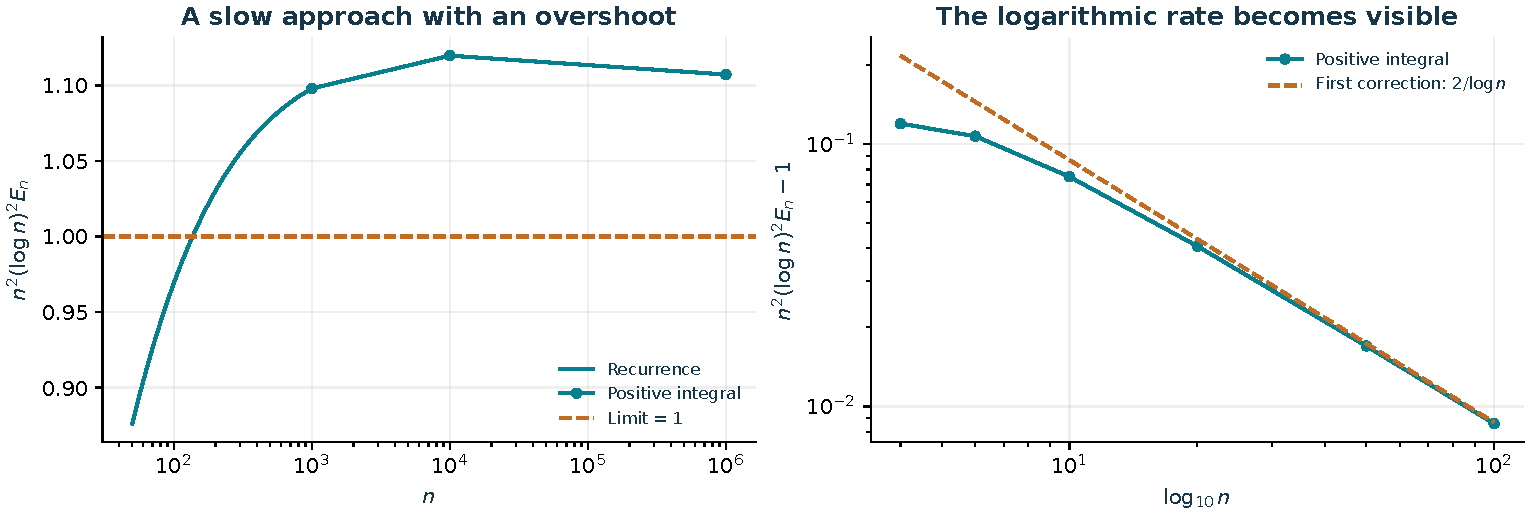
\includegraphics[width=\linewidth]{figures/normalized_remainder.pdf}
\caption{The finite-index approach and the eventual logarithmic rate.
The right horizontal axis is $\log_{10}n$, itself displayed on a
logarithmic scale. The curve $2/\log n$ is the first proved
relative correction, not a fitted model.}
\label{fig:normalized}
\end{figure}

Nor does a longer fixed inverse-logarithmic truncation always improve
a numerical approximation. For example, at $n=1000$, including
$c_0,\ldots,c_3$ gives relative error approximately
$-7.17\times10^{-4}$, whereas including $c_4$ as well gives
approximately $-1.67\times10^{-2}$. Asymptotic expansions assert
improvement as the limiting parameter tends to infinity at fixed
order, not a pointwise monotonic improvement with the order.

\subsection{Accuracy when the logarithmic integrals are retained}

Define the three successive approximations
\begin{align*}
 A_0(n)&=n^{-2}F_2(\log n),\\
 A_1(n)&=A_0(n)+(2n^3)^{-1}F_3(\log n),\\
 A_2(n)&=A_1(n)+n^{-4}
       \{F_4(\log n)/12-p_2F_4'(\log n)\}.
\end{align*}
Their errors, computed against the positive endpoint integral, are
shown in Table~\ref{tab:sectors}. The signs are retained in the table;
the plot uses absolute relative error. The next proved coefficient
in \eqref{eq:main-sectors} explains the remaining error of $A_2$.

\begin{table}[htbp]
\centering
\caption{Signed relative errors $A_j(n)/E_n-1$.}
\label{tab:sectors}
\begin{tabular}{@{}rrrr@{}}
\toprule
$n$ & $A_0$ & $A_1$ & $A_2$\\
\midrule
\tableinput data/table_sector_errors.tex
\bottomrule
\end{tabular}
\end{table}

\begin{figure}[htbp]
\centering
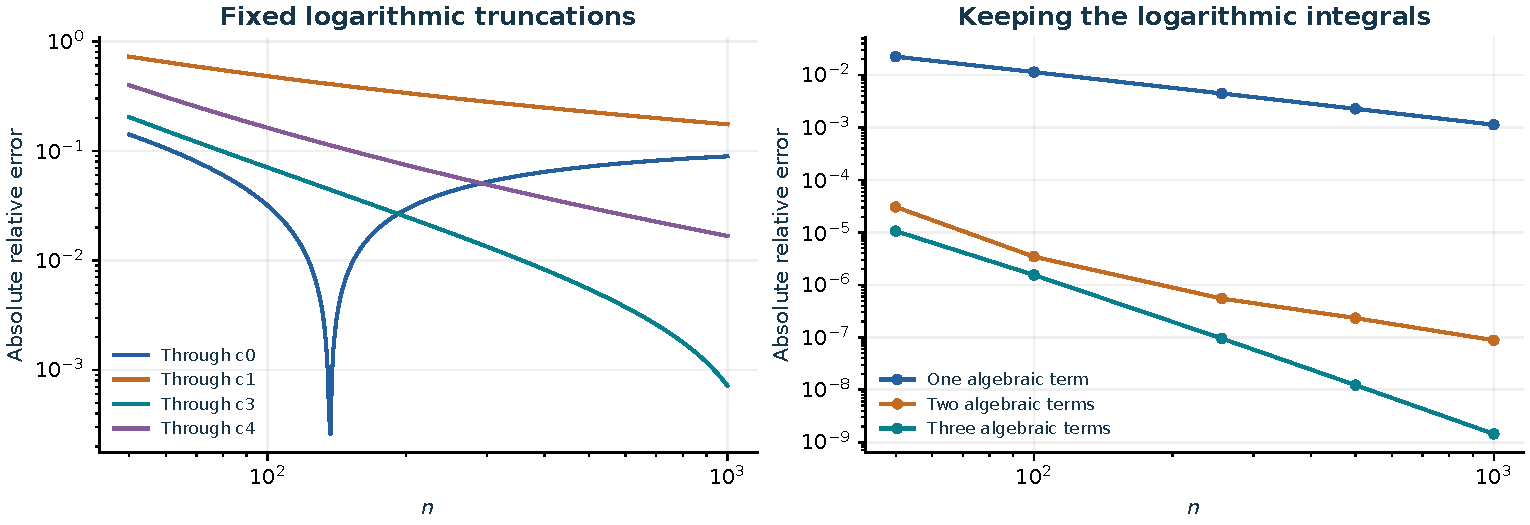
\includegraphics[width=\linewidth]{figures/approximation_errors.pdf}
\caption{Two types of approximation. On the left, a fixed number of
logarithmic terms may suffer cancellation or grow inaccurate at
moderate indices. On the right, the exact logarithmic integrals are
retained while successive powers of $1/n$ are added.}
\label{fig:errors}
\end{figure}

\subsection{The product constant}

The recorded finite product at $m=1000$ is
\[
 P_{1000}=0.61788133434828841381086077163828710263\ldots.
\]
The theorem proves that it lies above $C_*$, and
\eqref{eq:C-enclosure} provides an explicit tail enclosure in exact
arithmetic. The displayed decimal is a high-precision numerical
estimate of the finite product, rather than a certified decimal
enclosure of the infinite one.

\begin{table}[htbp]
\centering
\caption{Selected normalized partial products $P_m$, rounded by
truncating the displayed decimal expansion.}
\label{tab:product}
\begin{tabular}{@{}rl@{}}
\toprule
$m$ & $P_m$\\
\midrule
\tableinput data/table_product.tex
\bottomrule
\end{tabular}
\end{table}

\subsection{Reproduction commands and scope}

The Python programs require \texttt{mpmath}, \texttt{sympy},
\texttt{numpy}, \texttt{scipy}, and \texttt{matplotlib}. Versions
used in preparation are recorded in the data. From the package root:
\begin{verbatim}
python code/verify_recurrence.py --nmax 1000 --out rerun/data
python code/verify_symbolic.py --out rerun/symbolic_checks.json
python code/make_figures.py --input rerun/data --out rerun
make pdf
\end{verbatim}
The first three commands keep the originally supplied data intact.
Compilation uses the already included figures and tables, so building
the PDF does not require numerical libraries or network access.
Normal Python and optimized \texttt{python -O} runs produced the
same deterministic numerical data files in the preparation checks.
Runtime measurements and metadata are not expected to be identical
across machines.

\section{Further research questions and proposed next steps}
\label{sec:future}

The exact measure separates several questions that were difficult to
distinguish from the original recurrence. The following are concrete
extensions, with their unresolved parts stated explicitly.

\begin{enumerate}[leftmargin=*]
\item \textbf{Complete the priority comparison.}
Obtain the full Ford--Lau solution and inspect subsequent work on this
specific recurrence, including citations of the original problem.
Determine precisely which of the density formula, complete
monotonicity, all-orders coefficients, and product correction have
appeared before. This is the first step before describing the result
as a first publication.

\item \textbf{Optimal truncation of the inverse-logarithmic expansion.}
The coefficient generator is an entire reciprocal-gamma expression,
but the asymptotic coefficients also contain $(k+1)!$. Determine their
large-order behavior, the optimal truncation index as a function of
$\log n$, and the least attainable remainder for this single series.
The exact $F_a$ integrals provide a reference against which a proposed
optimal-truncation theorem can be tested. Fixed-order error estimates
in this paper do not answer this question.

\item \textbf{Uniformity when the algebraic order grows.}
Theorem~\ref{thm:main-sectors} and its general version hold for each
fixed truncation order. Quantify the dependence of the remainder
constant on that order, and determine a range $R=R(n)\to\infty$.
The singularities at distance $2\pi$ in the endpoint correction
$P$ are natural inputs, but the logarithmic denominator must be
controlled simultaneously.

\item \textbf{Interval-certified product constants and errors.}
Implement directed-rounding enclosures for $\rho$, $\gamma$, and
the positive integral. Combine them with
\eqref{eq:C-enclosure} or \eqref{eq:alternating-tail} to certify
the infinite product $C_*$ to an arbitrary requested number of digits.
An implementation should avoid subtraction of two exponentially large
terms. The current scripts demonstrate numerical agreement; they do
not provide these interval guarantees.

\item \textbf{Growing finite-difference order.}
The exact formula for $D_{n,r}$ remains valid for every $r$, whereas
\eqref{eq:difference-asymptotic} assumes fixed $r$. When $r/n$ stays
away from zero and infinity, its integral is controlled by an interior
beta-distribution saddle. Derive a uniform theorem joining that
interior regime to the logarithmic endpoint regime $r=o(n)$.
Such a theorem would describe the full array of difference inequalities,
not just each fixed column.

\item \textbf{General logarithmic renewal kernels.}
Suppose $a_{j+1}-a_j=\int_0^1t^{j-1}h(t)\,dt$ for a positive
density $h$, and $1+a_1\ge\int_0^1h(t)/t\,dt$.
Theorem~\ref{thm:general-kernel} gives an all-orders logarithmic
expansion under explicit regularity assumptions, with a possible atom
at zero. Determine minimal endpoint regularity for that conclusion,
and characterize precisely which deformations preserve the special
cancellation of Euler's constant in \eqref{eq:main-coeff}.
If $h(1)>0$ and a suitable logarithmic endpoint limit exists, the
same calculation predicts leading constant $1/h(1)$.

\item \textbf{Stability under perturbing initial coefficients.}
A finite change of the recurrence coefficients leaves their
logarithmic tail unchanged but may create additional poles.
Classify the perturbations for which the positive remainder measure
survives, and those for which oscillating exponential corrections
appear. The singularity at one should still determine a universal
logarithmic component after all relevant poles are removed; that
assertion requires a separate global zero analysis.

\item \textbf{Arithmetic error propagation.}
Insert the proved product correction into a fully audited
totient-volume argument and track every competing approximation.
Determine whether any arithmetic regime exposes the new
$\rho^m/(m^2\log^2m)$ scale rather than hiding it under a larger
sieve or boundary error. This paper proves the continuous-scale
correction and leaves that arithmetic comparison open.

\item \textbf{Lean formalization in stages.}
Start with the convolution recurrence, the integral formula for its
increments, and the algebraic relation between $G$ and $J$.
Next formalize the positive bounded operator and its scalar spectral
measure, including endpoint atoms. The exact moment inequalities
then follow with little asymptotic machinery. A final stage can
formalize the uniform Laplace estimates and coefficient extraction.
No declaration in the supplied package is represented as a
kernel-checked proof.
\end{enumerate}

\section{Integration and reproducibility record}
\label{sec:integration}

The package is self-contained for compilation and for the supplied
numerical experiments. It contains the complete LaTeX source, a
compiled PDF, vector figures and generated tables, Python programs,
CSV/JSON data, a build file, and a claim-status ledger. No original
repository manuscript or third-party PDF is redistributed.

The inspected repository snapshots were
\begin{center}\small
\begin{tabular}{@{}lp{0.71\linewidth}@{}}
\toprule
Repository & Commit\\
\midrule
\texttt{openai/math}&\path{adc7f1241b42e322a6451854ab7e4b4c146bf78a}\\
\texttt{ProveIt}&\path{6d78805163d6b5b92d27f8f41555254c49fe0963}\\
\bottomrule
\end{tabular}
\end{center}
The first snapshot supplies the recurrence and product-scale anchor;
the second records the repository scope at the start of the study.
Their full paths and the relevant source blob identifier appear in
\texttt{provenance.json}. The inspection was targeted, and did not
constitute a theorem-by-theorem audit of either repository.

An appropriate proposed destination is
\path{Analysis/RenewalTheory/Research/Ford_Renewal_Logarithmic_Remainder/}.
This is an integration suggestion; no existing repository content has
been changed or published by this package.

The mathematical dependency is short: a positive operator gives the
exact residual measure; elementary endpoint estimates give its sharp
size and explicit bounds; a convergent polylogarithm identity gives
the complete expansions; positive integral identities transport them
to products and renewal accuracy. The numerical programs check each
description against an independently computed representation. Their
purpose is reproducibility and error detection, while the proofs above
establish the infinite statements.

\begin{thebibliography}{9}

\bibitem{Ford}
K. Ford, \emph{The distribution of totients},
Ramanujan J. \textbf{2} (1998), 67--151.
The version used here is the revised manuscript
\href{https://arxiv.org/abs/1104.3264v2}{arXiv:1104.3264v2}
(14 July 2013), especially Section~3, Lemma~3.7 and Remark~1.
Author's PDF:
\url{https://www.ford126.web.illinois.edu/wwwpapers/totients.pdf}.

\bibitem{FordLau}
K. Ford and K.-W. Lau, \emph{Problems and Solutions: Solutions:
Asymptotics of a Recurrent Sequence: 10682},
Amer. Math. Monthly \textbf{107}(4) (2000), 374--375.
\href{https://doi.org/10.2307/2589199}{doi:10.2307/2589199}.
Bibliographic identification checked against the University of Illinois
publication record; the full text was not inspected. The year 2000
is used here rather than the year printed in reference [17] of
the revised Ford manuscript.

\bibitem{DLMF}
F. W. J. Olver et al., eds., \emph{NIST Digital Library of Mathematical
Functions}. Section~25.12, especially equation~25.12.12 (convergent
polylogarithm expansion), and Section~5.7 (gamma-function series).
\url{https://dlmf.nist.gov/25.12} and
\url{https://dlmf.nist.gov/5.7}. Accessed 8 October 2026.

\bibitem{Teschl}
G. Teschl, \emph{Topics in Linear and Nonlinear Functional Analysis},
author's textbook page and contents, especially the spectral theorem
and spectral measures in Chapter~5.
\url{https://www.mat.univie.ac.at/~gerald/ftp/book-fa/fa.html}.
The general bounded self-adjoint spectral theorem is the standard
functional-analytic input used in Section~\ref{sec:spectral-notes}.

\bibitem{OpenAIMath}
OpenAI, \emph{An asymptotic formula for the number of totients},
repository manuscript dated 25 September 2026, in \texttt{openai/math}.
Inspected source:
\path{preprints/An-asymptotic-formula-for-the-number-of-totients-September-25-2026/build/source/statements.tex},
commit \path{adc7f1241b42e322a6451854ab7e4b4c146bf78a}.
\url{https://github.com/openai/math}.
Only the explicitly defined recurrence and product scale are used here;
the manuscript's main arithmetic theorem is not an input.

\bibitem{ProveIt}
V. Reshetnikov, \emph{ProveIt}, research and formal-mathematics repository,
snapshot \path{6d78805163d6b5b92d27f8f41555254c49fe0963}.
\url{https://github.com/VladimirReshetnikov/ProveIt}.
The inspected asymptotic and conditioning material was used to select
a nonduplicative direction, not as an unproved lemma in this article.

\end{thebibliography}

\end{document}
